\chapter{Additional figures}
\label{ch:results_appendix}

\section{Tabular}

%Tabular benchmarks for joint architecture and hyperparameter optimization. Klein, A. and Hutter, F. 2019.
\begin{figure}[H]
    \centering
    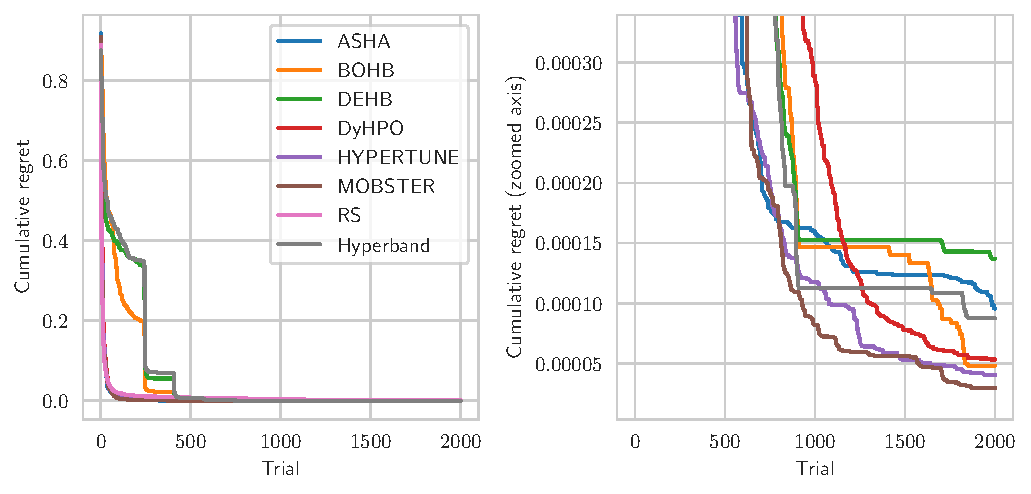
\includegraphics[scale=0.65]{img/tabular_exp/fcnet-naval_plot.pdf}
    \caption{Results of the fcnet-naval experiment.}
    %\label{}
\end{figure}

\begin{figure}[H]
    \centering
    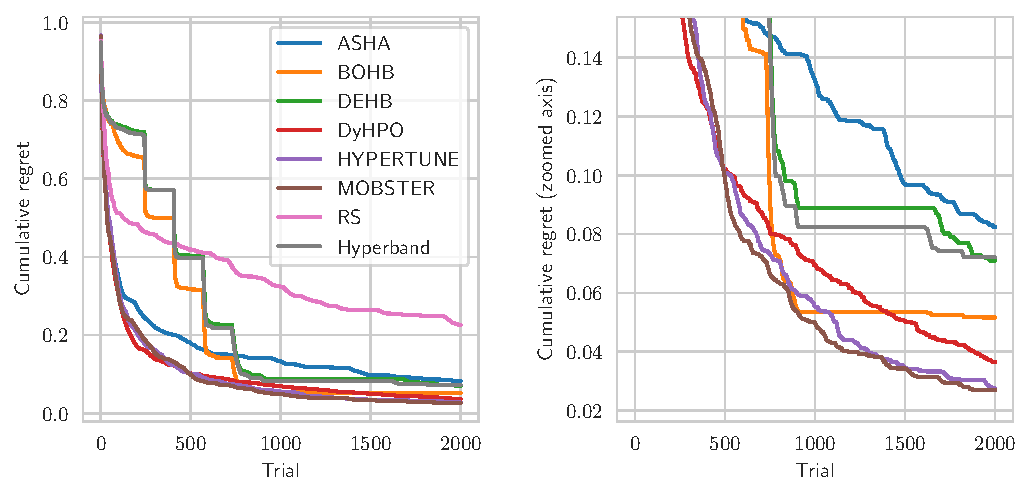
\includegraphics[scale=0.65]{img/tabular_exp/fcnet-protein_plot.pdf}
    \caption{Results of the fcnet-protein experiment.}
    %\label{}
\end{figure}


\begin{figure}[H]
    \centering
    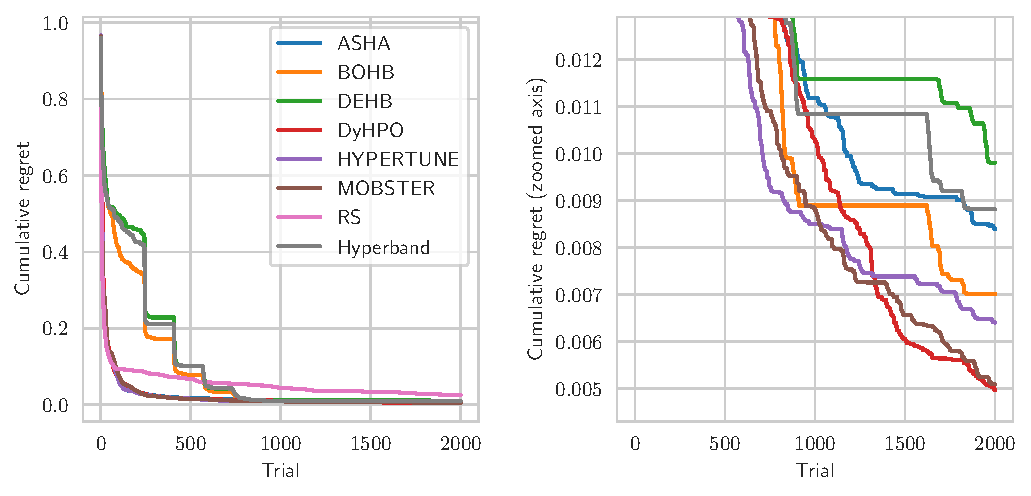
\includegraphics[scale=0.65]{img/tabular_exp/fcnet-parkinsons_plot.pdf}
    \caption{Results of the fcnet-parkinsons experiment.}
    %\label{}
\end{figure}

\begin{figure}[H]
    \centering
    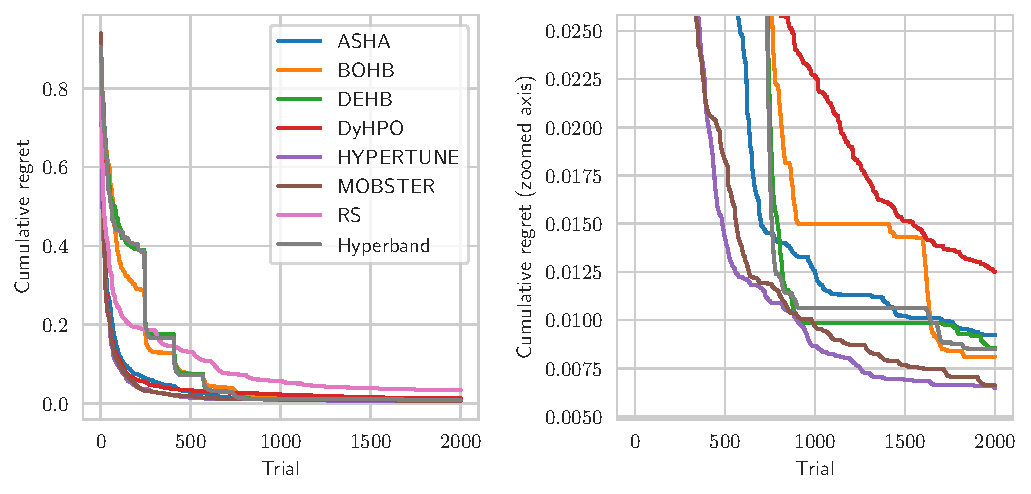
\includegraphics[scale=0.65]{img/tabular_exp/fcnet-slice_plot.pdf}
    \caption{Results of the fcnet-slice experiment.}
    %\label{}
\end{figure}




% NAS-Bench-201: Extending the scope of reproducible neural architecture search. Dong, X. and Yang, Y. 2020.
\begin{figure}[H]
    \centering
    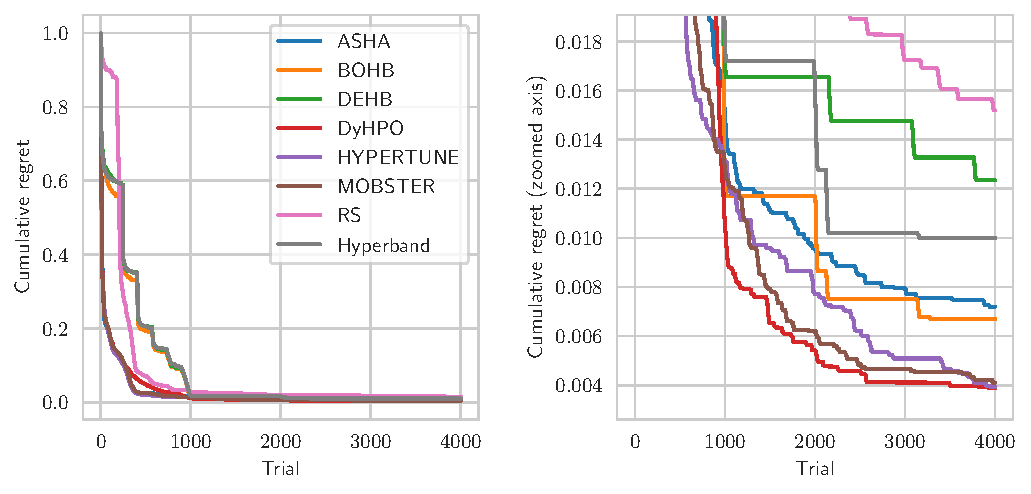
\includegraphics[scale=0.65]{img/tabular_exp/nas201-cifar10_plot.pdf}
    \caption{Results of the nas201-cifar10 experiment.}
    %\label{}
\end{figure}

\begin{figure}[H]
    \centering
    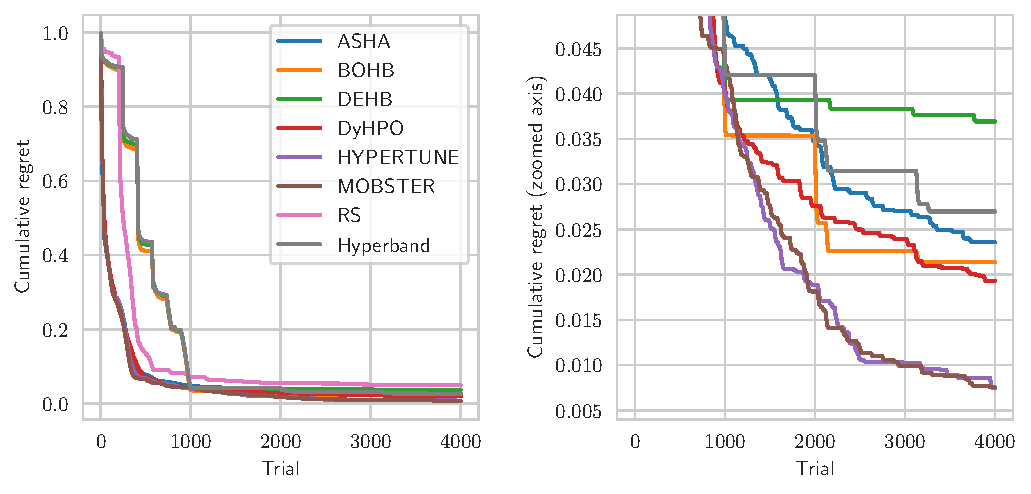
\includegraphics[scale=0.65]{img/tabular_exp/nas201-cifar100_plot.pdf}
    \caption{Results of the nas201-cifar100 experiment.}
    %\label{}
\end{figure}

\begin{figure}[H]
    \centering
    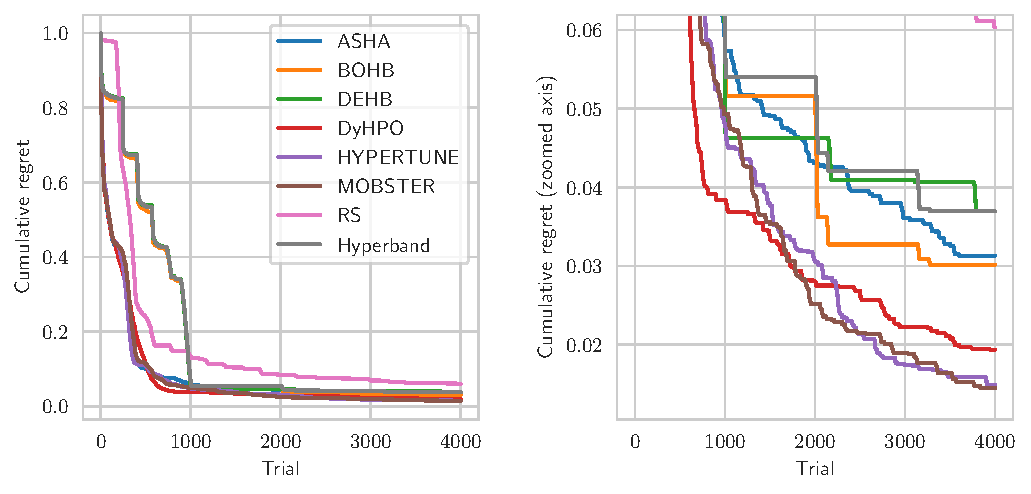
\includegraphics[scale=0.65]{img/tabular_exp/nas201-ImageNet16-120_plot.pdf}
    \caption{Results of the nas201-ImageNet16-120 experiment.}
    %\label{}
\end{figure}

%Reference: Auto-PyTorch: Multi-Fidelity MetaLearning for Efficient and Robust AutoDL. Lucas Zimmer, Marius Lindauer, Frank Hutter. 2020.
\begin{figure}[H]
    \centering
    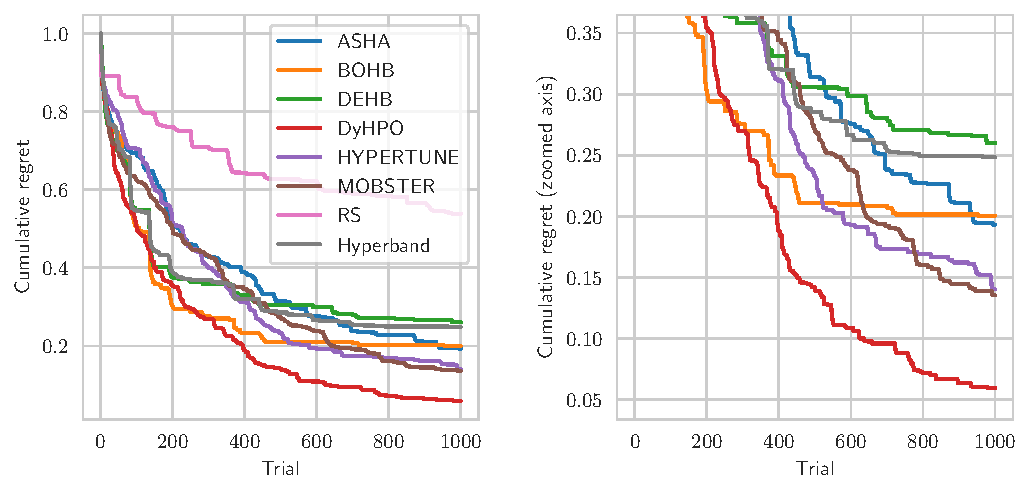
\includegraphics[scale=0.65]{img/tabular_exp/lcbench-airlines_plot.pdf}
    \caption{Results of the lcbench-airlines experiment.}
    %\label{}
\end{figure}

\begin{figure}[H]
    \centering
    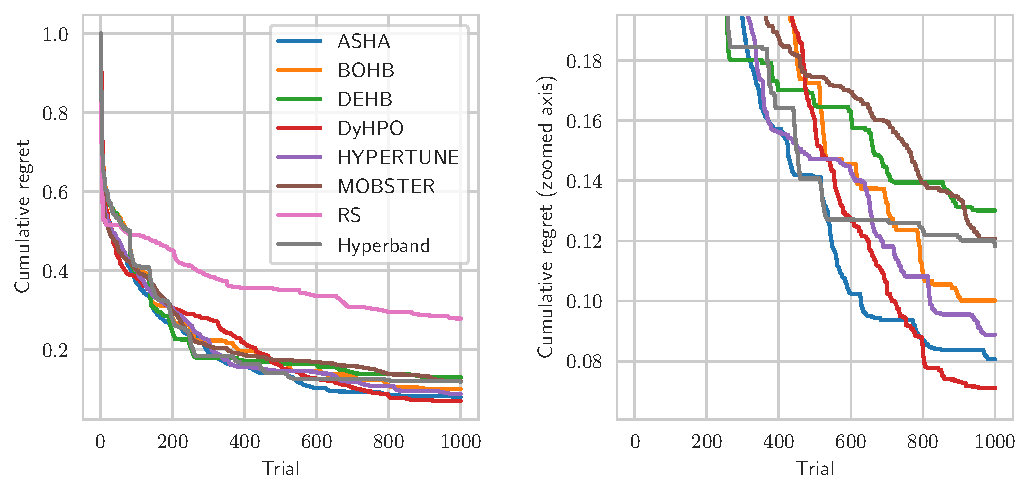
\includegraphics[scale=0.65]{img/tabular_exp/lcbench-albert_plot.pdf}
    \caption{Results of the lcbench-albert experiment.}
    %\label{}
\end{figure}

\begin{figure}[H]
    \centering
    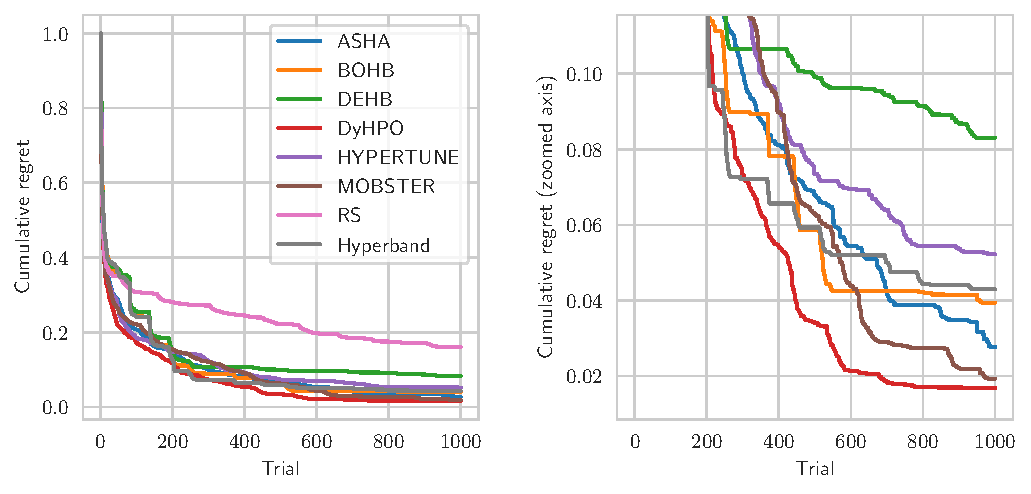
\includegraphics[scale=0.65]{img/tabular_exp/lcbench-Fashion-MNIST_plot.pdf}
    \caption{Results of the lcbench-Fashion-MNIST experiment.}
    %\label{}
\end{figure}

\begin{figure}[H]
    \centering
    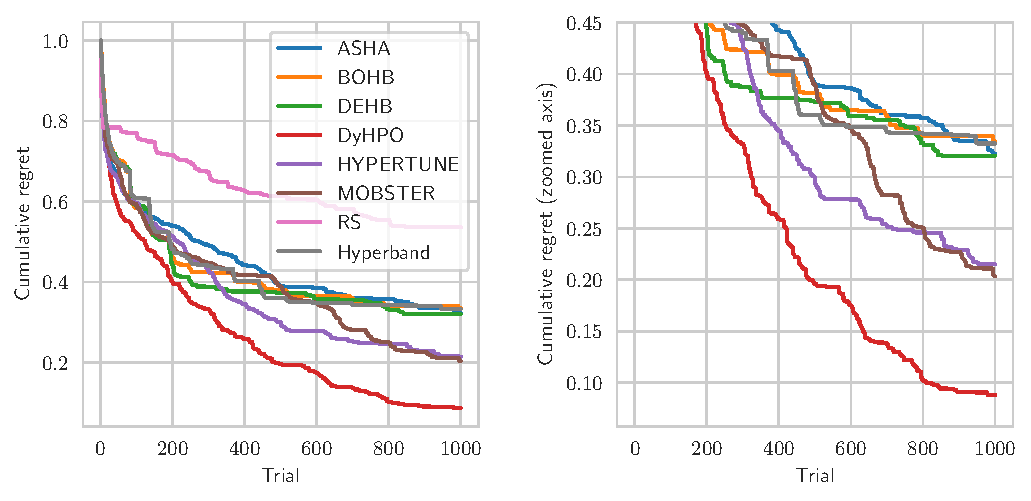
\includegraphics[scale=0.65]{img/tabular_exp/lcbench-covertype_plot.pdf}
    \caption{Results of the lcbench-covertype experiment.}
    %\label{}
\end{figure}

\begin{figure}[H]
    \centering
    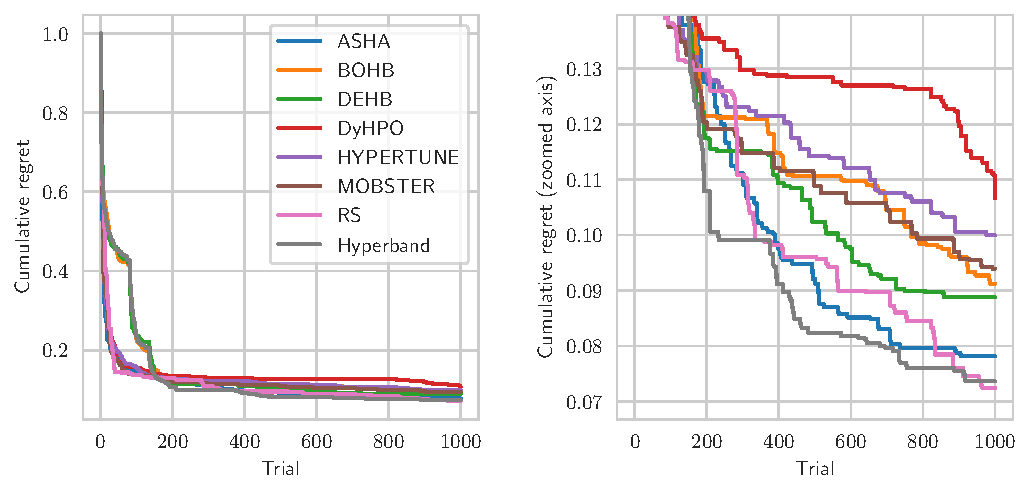
\includegraphics[scale=0.65]{img/tabular_exp/lcbench-christine_plot.pdf}
    \caption{Results of the lcbench-christine experiment.}
    %\label{}
\end{figure}

\begin{figure}[H]
    \centering
    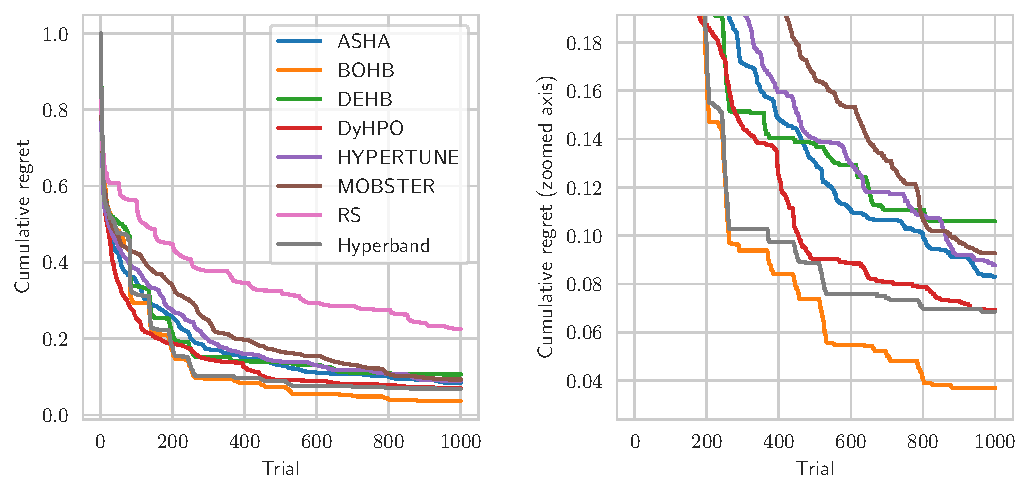
\includegraphics[scale=0.65]{img/tabular_exp/lcbench-higgs_plot.pdf}
    \caption{Results of the lcbench-higgs experiment.}
    %\label{}
\end{figure}

\begin{figure}[H]
    \centering
    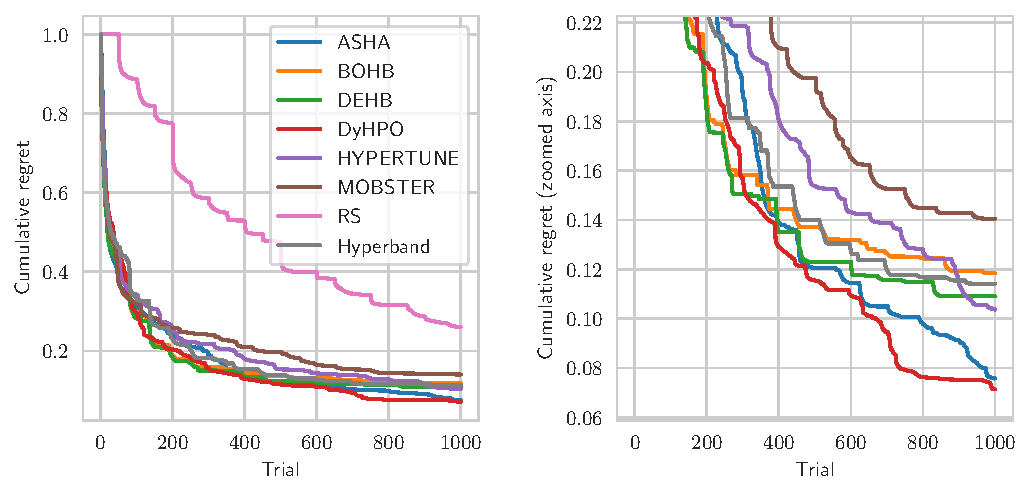
\includegraphics[scale=0.65]{img/tabular_exp/lcbench-dionis_plot.pdf}
    \caption{Results of the lcbench-dionis experiment.}
    %\label{}
\end{figure}

\begin{figure}[H]
    \centering
    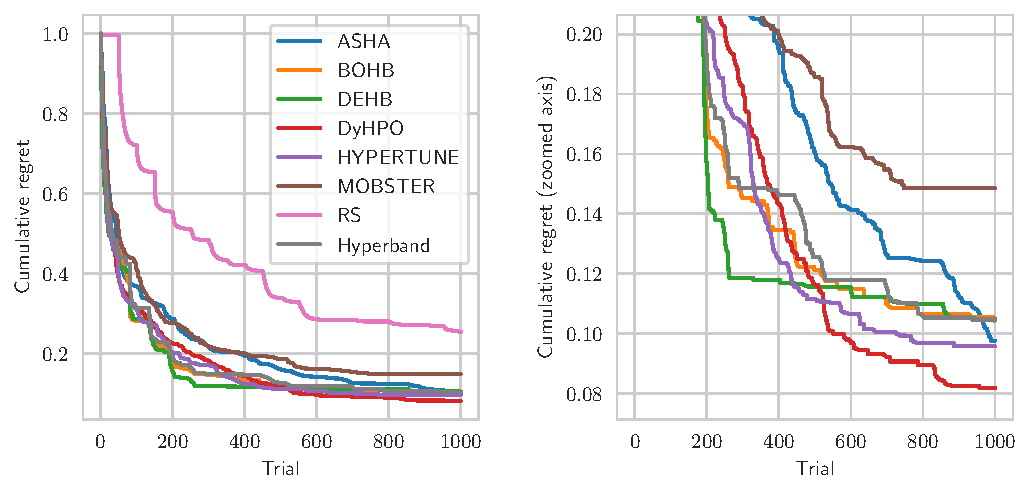
\includegraphics[scale=0.65]{img/tabular_exp/lcbench-helena_plot.pdf}
    \caption{Results of the lcbench-helena experiment.}
    %\label{}
\end{figure}


\section{Real-world}


\begin{figure}[H]
    \centering
    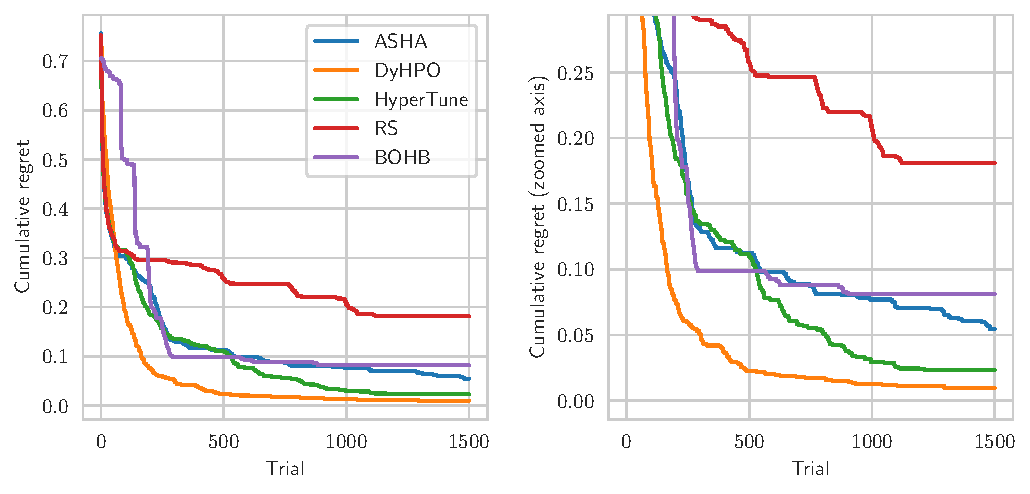
\includegraphics[scale=0.65]{img/real_exp/cifar10_simple_regret_plot.pdf}
    \caption{Results of the cifar10-cnn experiment.}
    \label{fig:cifar10_simple}
\end{figure}

\begin{figure}[H]
    \centering
    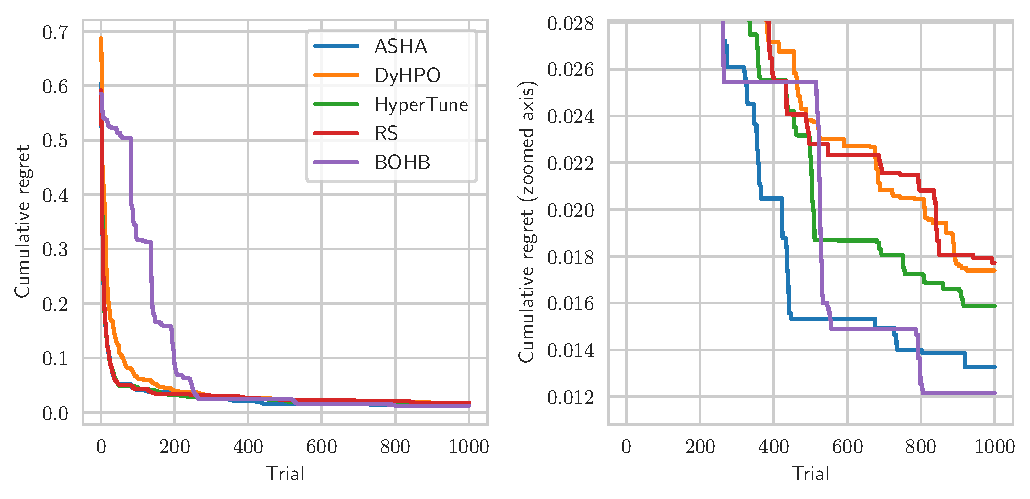
\includegraphics[scale=0.65]{img/real_exp/cifar10_residual_regret_plot.pdf}
    \caption{Results of the cifar10-residual experiment.}
    \label{fig:cifar10_residual}
\end{figure}

\begin{figure}[H]
    \centering
    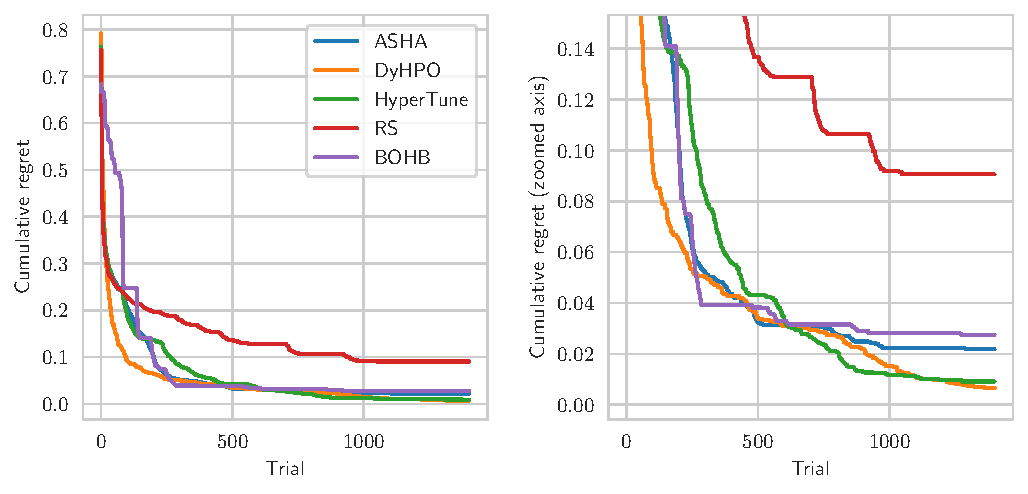
\includegraphics[scale=0.65]{img/real_exp/svhn_simple_regret_plot.pdf}
    \caption{Results of the svhn-cnn experiment.}
    \label{fig:svhn_simple}
\end{figure}

\begin{figure}[H]
    \centering
    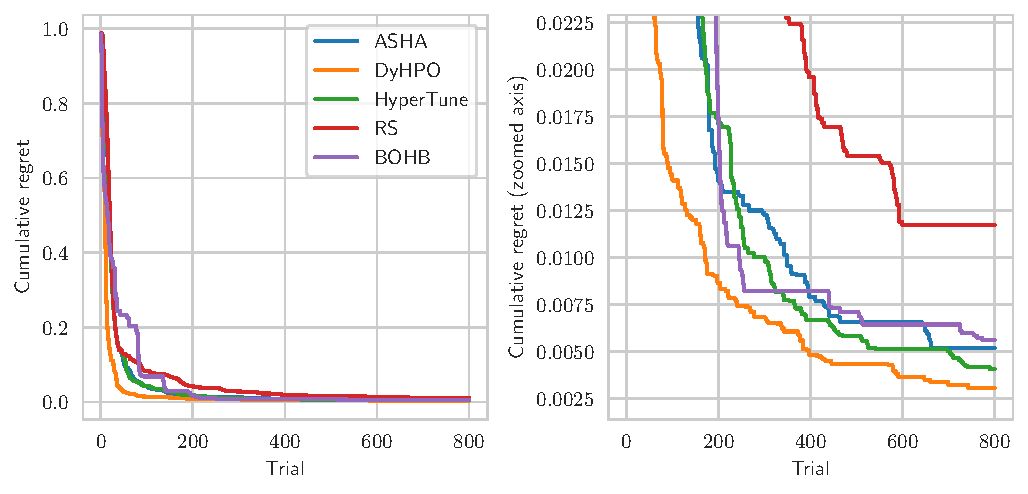
\includegraphics[scale=0.65]{img/real_exp/svhn_residual_regret_plot.pdf}
    \caption{Results of the svhn-residual experiment.}
    \label{fig:svhn_residual}
\end{figure}


\begin{figure}[H]
    \centering
    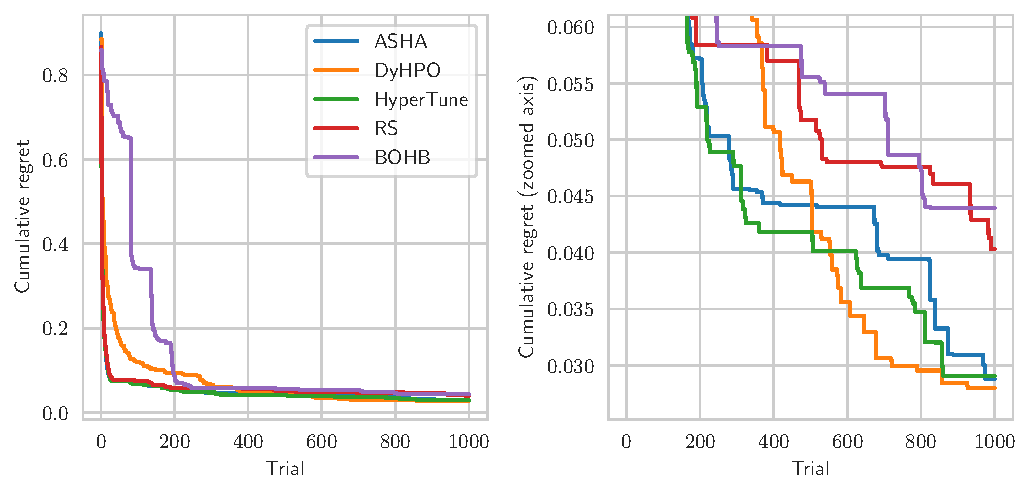
\includegraphics[scale=0.65]{img/real_exp/ptbxl_rnn_regret_plot.pdf}
    \caption{Results of the ptbxl-rnn experiment.}
    \label{fig:ptbxl_rnn}
\end{figure}

\begin{figure}[H]
    \centering
    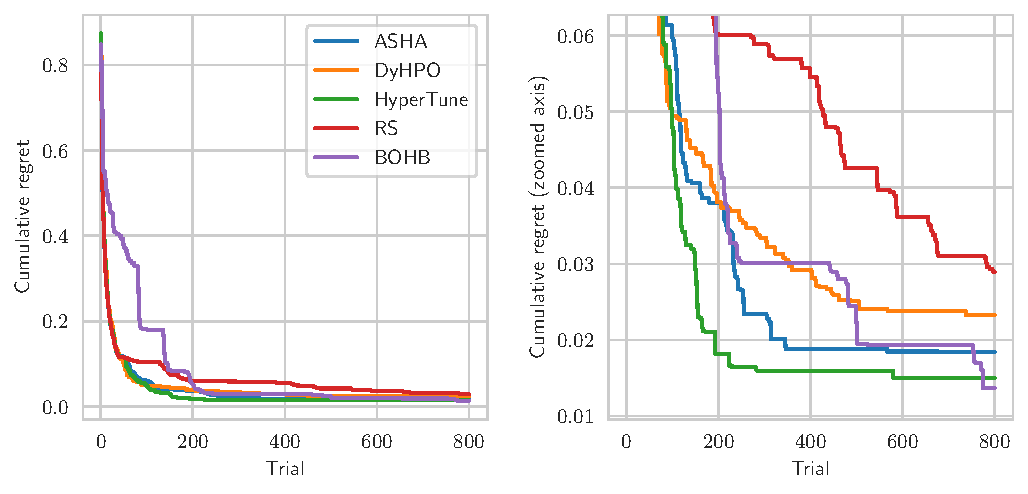
\includegraphics[scale=0.65]{img/real_exp/ptbxl_xResNet1d_regret_plot.pdf}
    \caption{Results of the ptbxl-xResnet1d experiment.}
    \label{fig:ptbxl_xresnet}
\end{figure}

\begin{figure}[H]
    \centering
    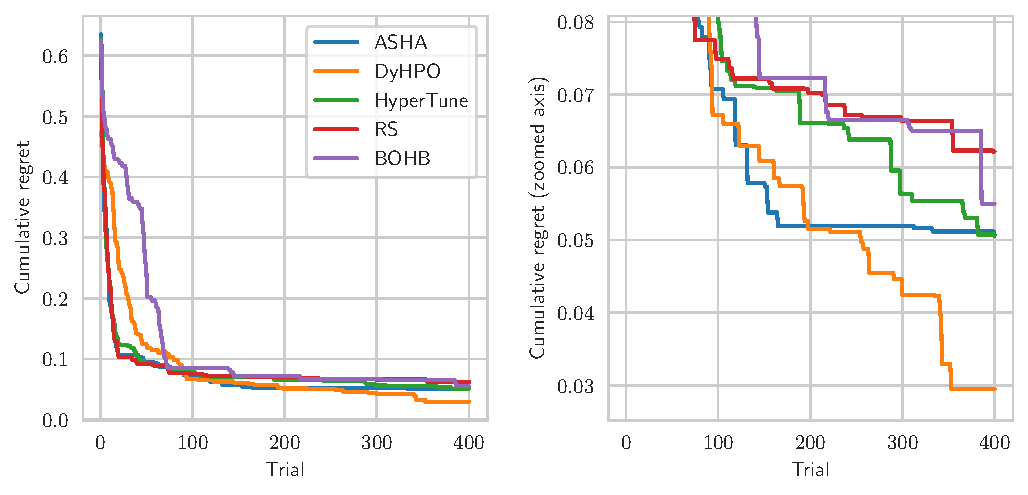
\includegraphics[scale=0.65]{img/real_exp/xray_densenet_regret_plot.pdf}
    \caption{Results of the xray-densenet experiment.}
    \label{fig:xray_densenet}
\end{figure}
